\documentclass{article}
\usepackage{tikz}
\usetikzlibrary{positioning, arrows.meta, fit, backgrounds}



\begin{document}
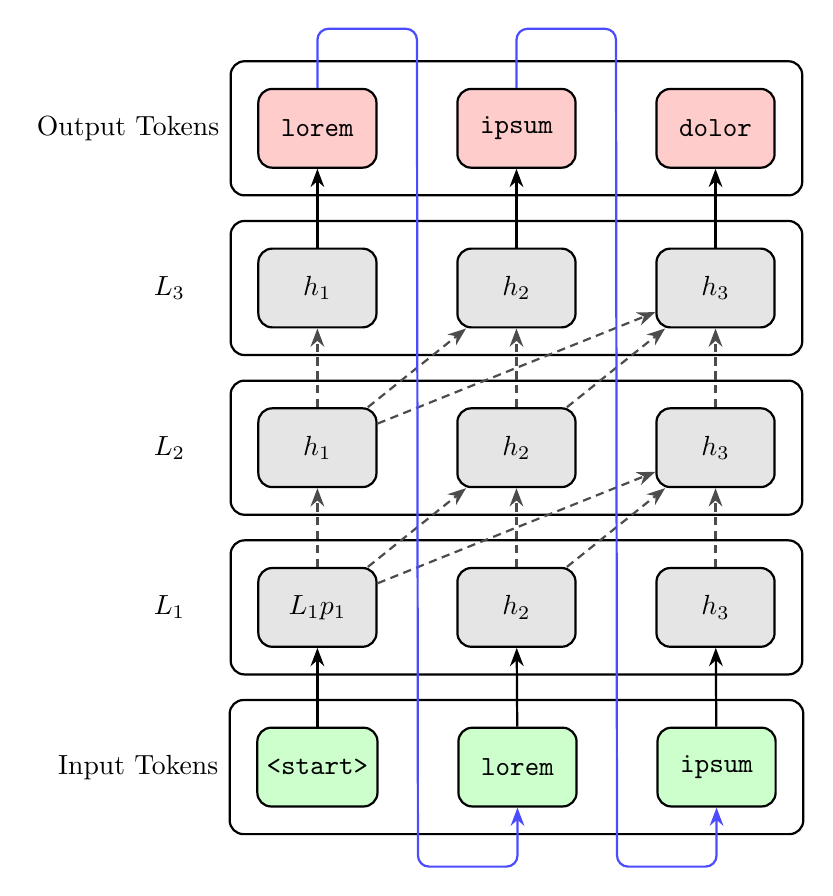
\begin{tikzpicture}[node distance=1cm and 1cm, >=Stealth, thick,
    every node/.style={draw, minimum width=1.5cm, minimum height=1cm, align=center, rounded corners=5pt},
    input/.style={fill=green!20},
    output/.style={fill=red!20},
    hidden/.style={fill=gray!20},
    attention/.style={->, draw=black!70, thick, densely dashed},
    recurrence/.style={->, draw=blue!70, thick, rounded corners}]


% Nodes for input layer
\begin{scope}[local bounding box=input box]
    \node[input] (x1) {\tt{<start>}};
    \node[input, right=of x1] (x2) {\tt{lorem}};
    \node[input, right=of x2] (x3) {\tt{ipsum}};
\end{scope}
\node[fit=(input box), draw, label=left:Input Tokens, inner sep=10pt] {};

% Nodes for hidden layer L1
\begin{scope}[local bounding box=l1 box]
    \node[hidden, above=of   x1] (l1h1) {$L_{1}p_1$}; %this one is marked
    \node[hidden, right=of l1h1] (l1h2) {$h_2$};
    \node[hidden, right=of l1h2] (l1h3) {$h_3$};
\end{scope}
\node[fit=(l1 box), draw, label=left:$L_1$, inner sep=10pt] {};

% Nodes for hidden layer L2
\begin{scope}[local bounding box=l2 box]
    \node[hidden, above=of l1h1] (l2h1) {$h_1$};
    \node[hidden, right=of l2h1] (l2h2) {$h_2$};
    \node[hidden, right=of l2h2] (l2h3) {$h_3$};
\end{scope}
\node[fit=(l2 box), draw, label=left:$L_2$, inner sep=10pt] {};

% Nodes for hidden layer L3
\begin{scope}[local bounding box=l3 box]
    \node[hidden, above=of l2h1] (l3h1) {$h_1$};
    \node[hidden, right=of l3h1] (l3h2) {$h_2$};
    \node[hidden, right=of l3h2] (l3h3) {$h_3$};
\end{scope}
\node[fit=(l3 box), draw, label=left:$L_3$, inner sep=10pt] {};

% Nodes for output layer
\begin{scope}[local bounding box=output box]
    \node[output, above=of l3h1] (y1) {\tt{lorem}};
    \node[output, right=of y1] (y2) {\tt{ipsum}};
    \node[output, right=of y2] (y3) {\tt{dolor}};
\end{scope}
\node[fit=(output box), draw, label=left:Output Tokens, inner sep=10pt] {};

% input tokens to L1
\draw[->] (x1) -- (l1h1);
\draw[->] (x2) -- (l1h2);
\draw[->] (x3) -- (l1h3);

% attention connections from L1 to L2
\draw[attention] (l1h1) -- (l2h1);
\draw[attention] (l1h1) -- (l2h2);
\draw[attention] (l1h1) -- (l2h3);
\draw[attention] (l1h2) -- (l2h2);
\draw[attention] (l1h2) -- (l2h3);
\draw[attention] (l1h3) -- (l2h3);

% attention connections from L2 to L3
\draw[attention] (l2h1) -- (l3h1);
\draw[attention] (l2h1) -- (l3h2);
\draw[attention] (l2h1) -- (l3h3);
\draw[attention] (l2h2) -- (l3h2);
\draw[attention] (l2h2) -- (l3h3);
\draw[attention] (l2h3) -- (l3h3);

% final hidden layer to output tokens
\draw[->] (l3h1) -- (y1);
\draw[->] (l3h2) -- (y2);
\draw[->] (l3h3) -- (y3);

% autoregressive recurrence

% Draw the recurrence connections with waypoints
\node[coordinate, above right=0.75cm and 0.5cm of y1] (p1o) {};
\node[coordinate, below right=0.75cm and 0.5cm of x1] (p1i) {};
\draw[recurrence] (y1.north) |- (p1o) -- (p1i) -| (x2.south);

\node[coordinate, above right=0.75cm and 0.5cm of y2] (p2o) {};
\node[coordinate, below right=0.75cm and 0.5cm of x2] (p2i) {};
\draw[recurrence] (y2.north) |- (p2o) -- (p2i) -| (x3.south);

\end{tikzpicture}
\end{document}
